\documentclass[9pt]{article}
\usepackage[spanish]{babel}
\usepackage[utf8]{inputenc}
\usepackage{graphicx}
\graphicspath{{media/}}
\usepackage{caption}
\captionsetup{labelformat=empty}
%\renewcommand{\familydefault}{\sfdefault}
\title{Proyecto 1}
\author{Carlos Gerardo Acosta Hernández \\ Andrea Itzel González Vargas \\ Luis Pablo Mayo Vega}
\date{Redes de Computadoras\\Facultad de Ciencias, UNAM}
\setlength{\parindent}{0em}
\begin{document}
\maketitle

\section*{Reporte}

\subsection*{Diagrama de Red}

\subsection*{DNS}
Se muestran capturas de pantalla de las configuraciones de \textit{nameservers} y los registros \textsf{DNS} usados.\\
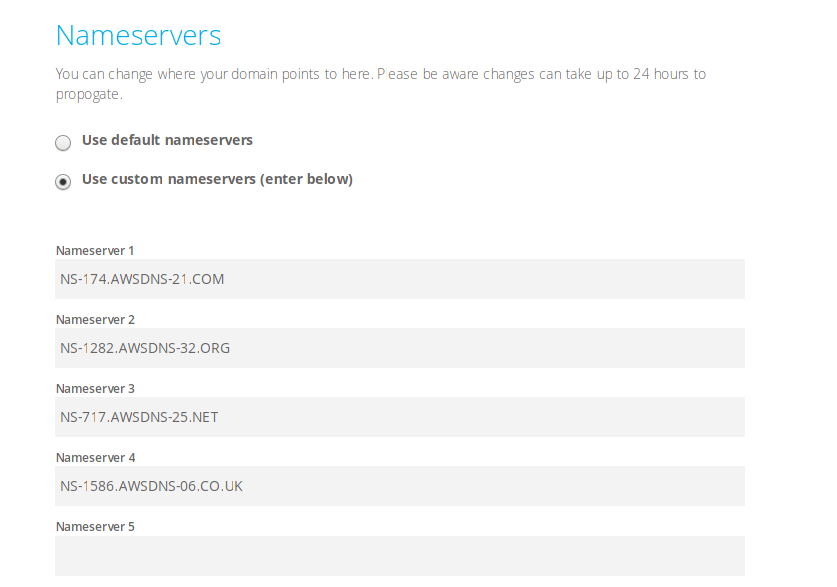
\includegraphics[width=\textwidth]{nameservers}
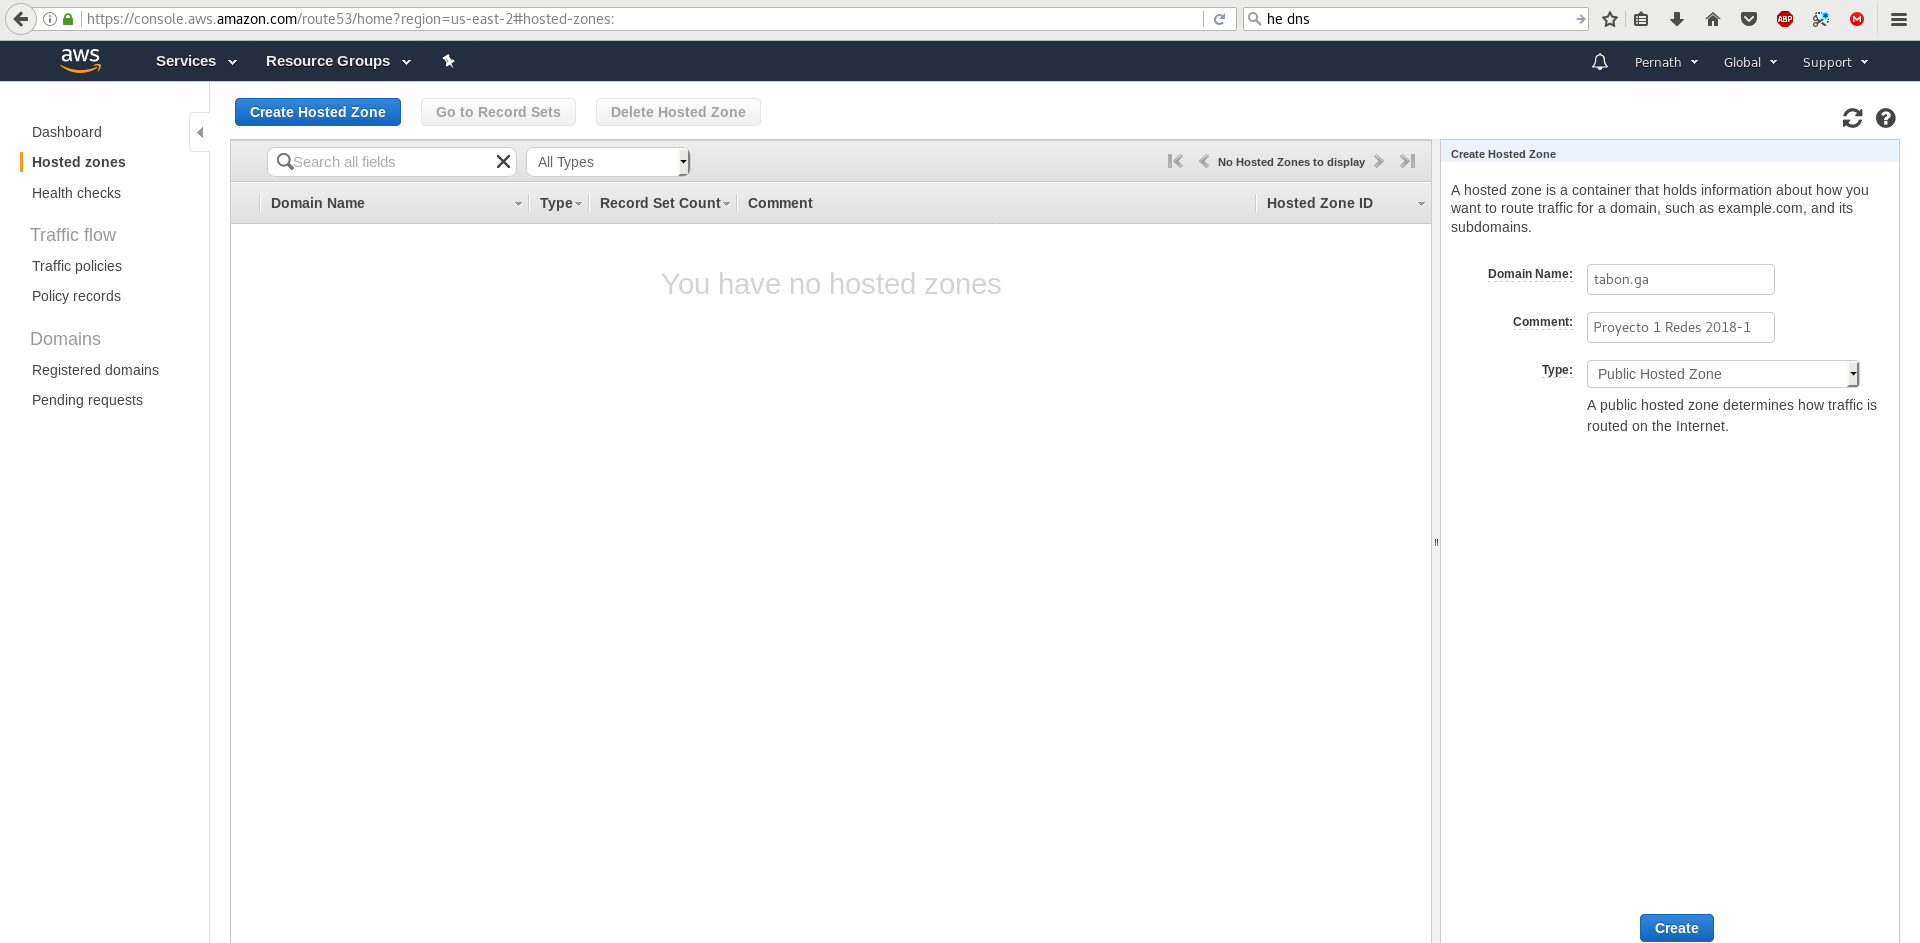
\includegraphics[width=\textwidth]{DNS_management}
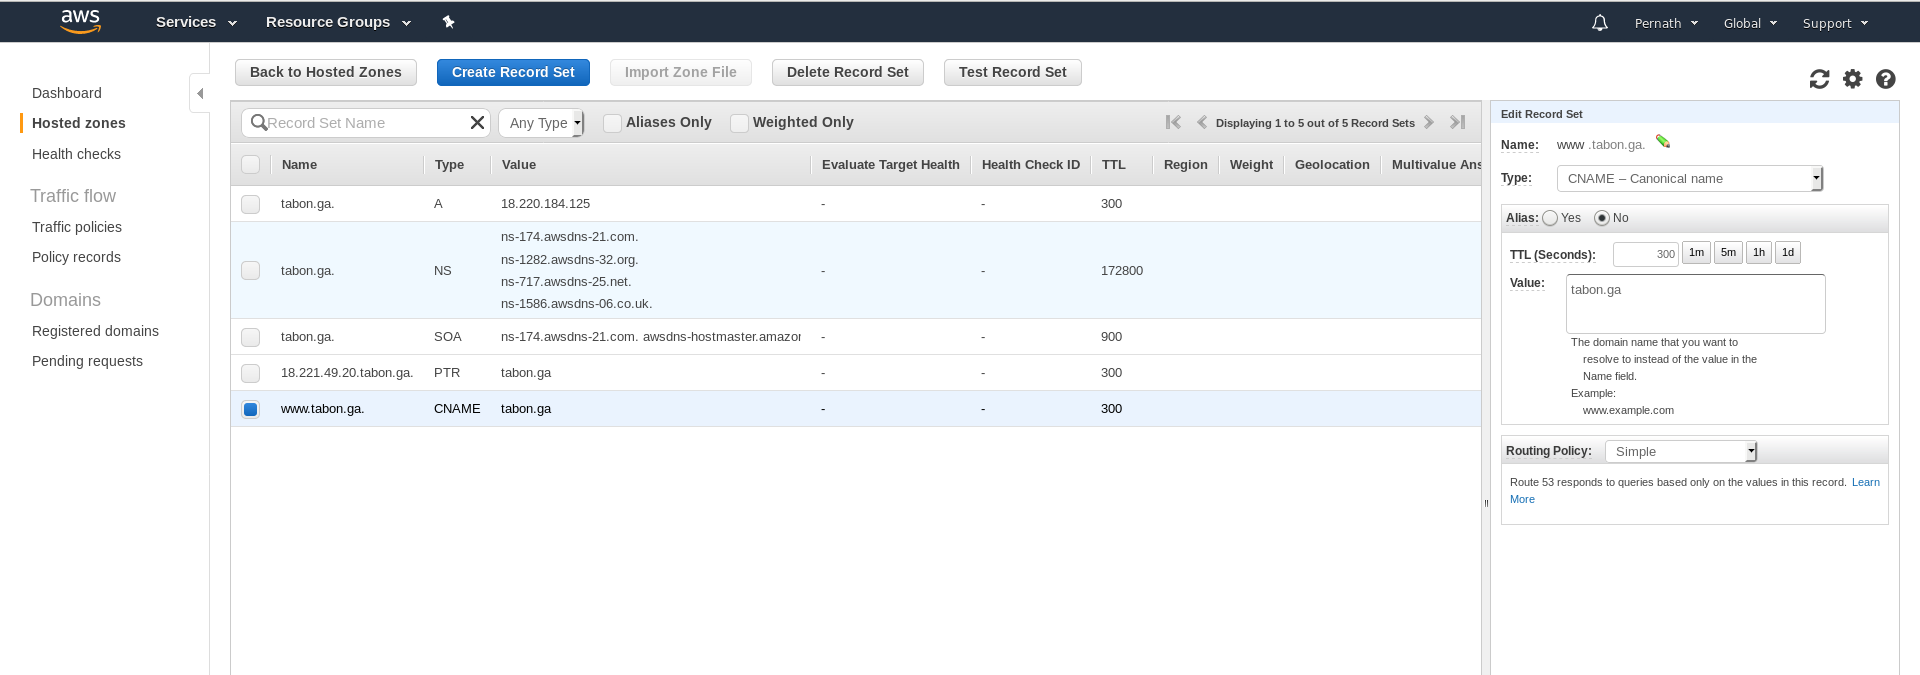
\includegraphics[width=\textwidth]{CNAME}
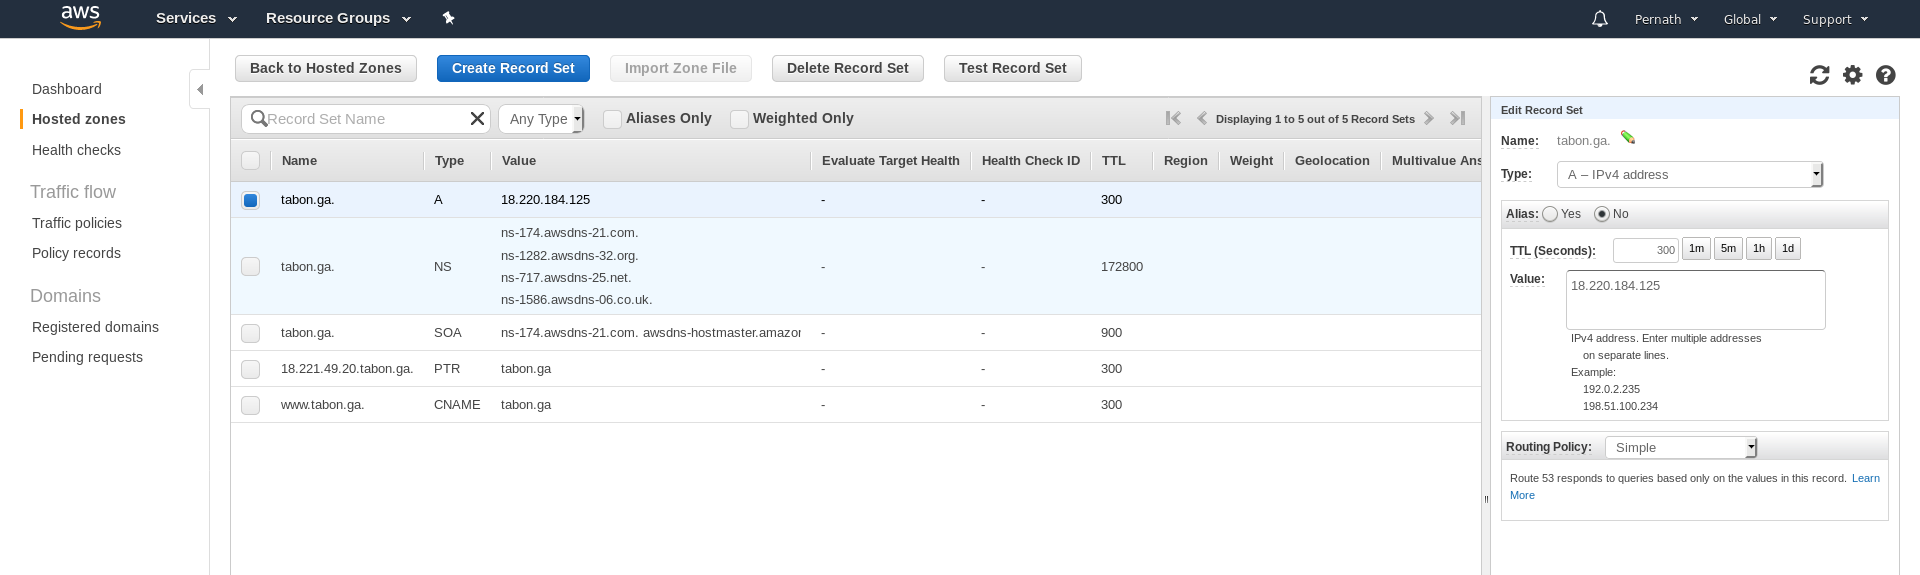
\includegraphics[width=\textwidth]{A}
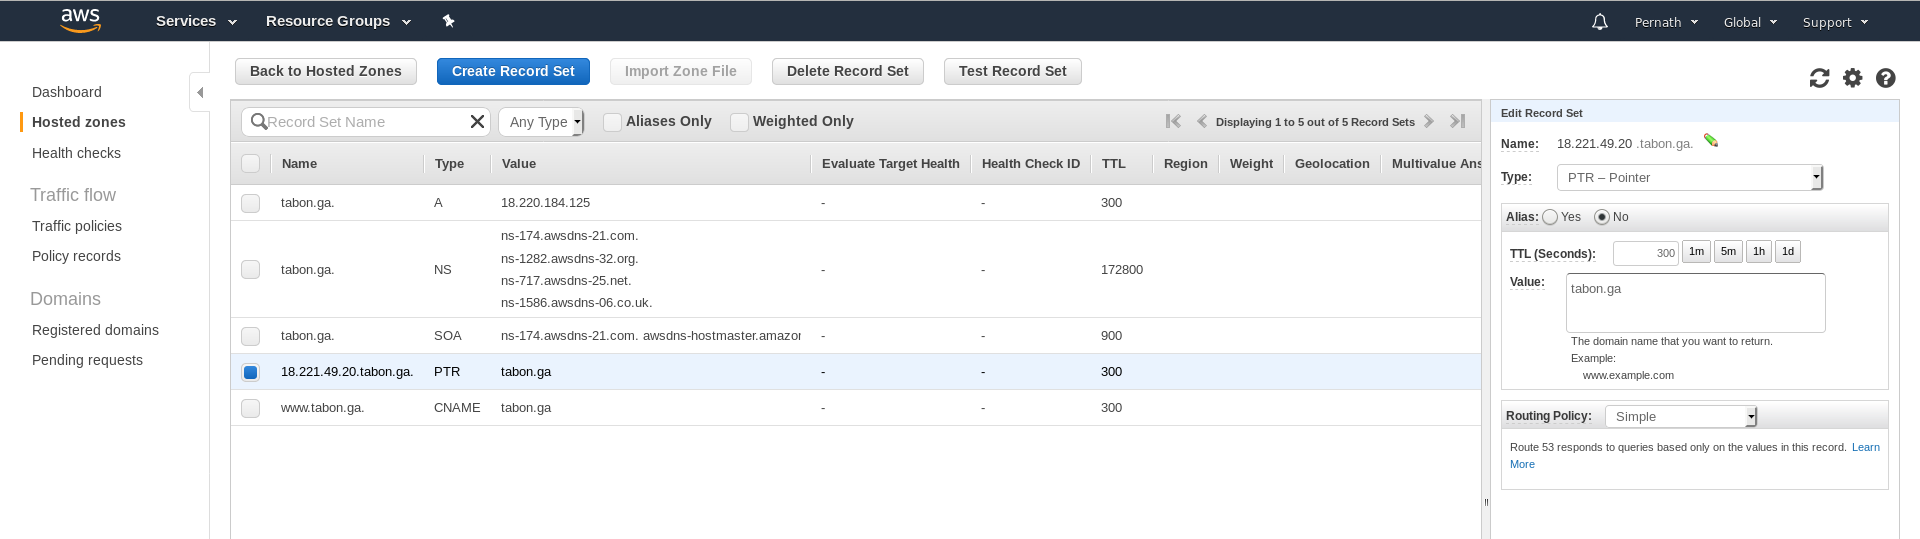
\includegraphics[width=\textwidth]{PTR}
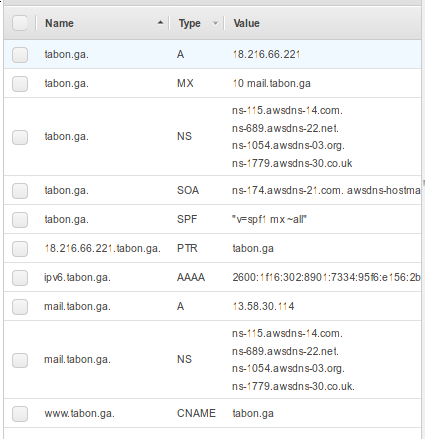
\includegraphics[width=\textwidth]{record_set}

\subsection*{Resumen de las configuraciones del servidor web y el servidor de aplicación y base de datos}
Se muestran capturas de pantalla de las configuraciones realizadas desde Amazon y vía \textsf{ssh} para las VPC, así como los certificados para \textsf{HTTPS/SSL} en ambos servidores.\\
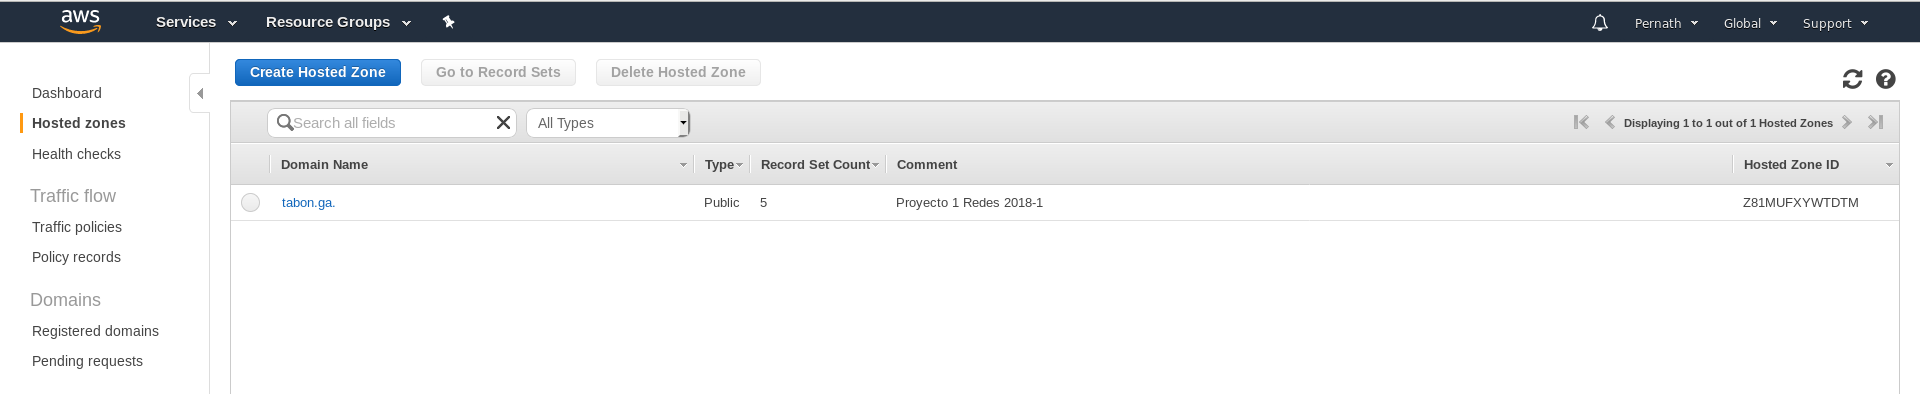
\includegraphics[width=\textwidth]{HostedZones}
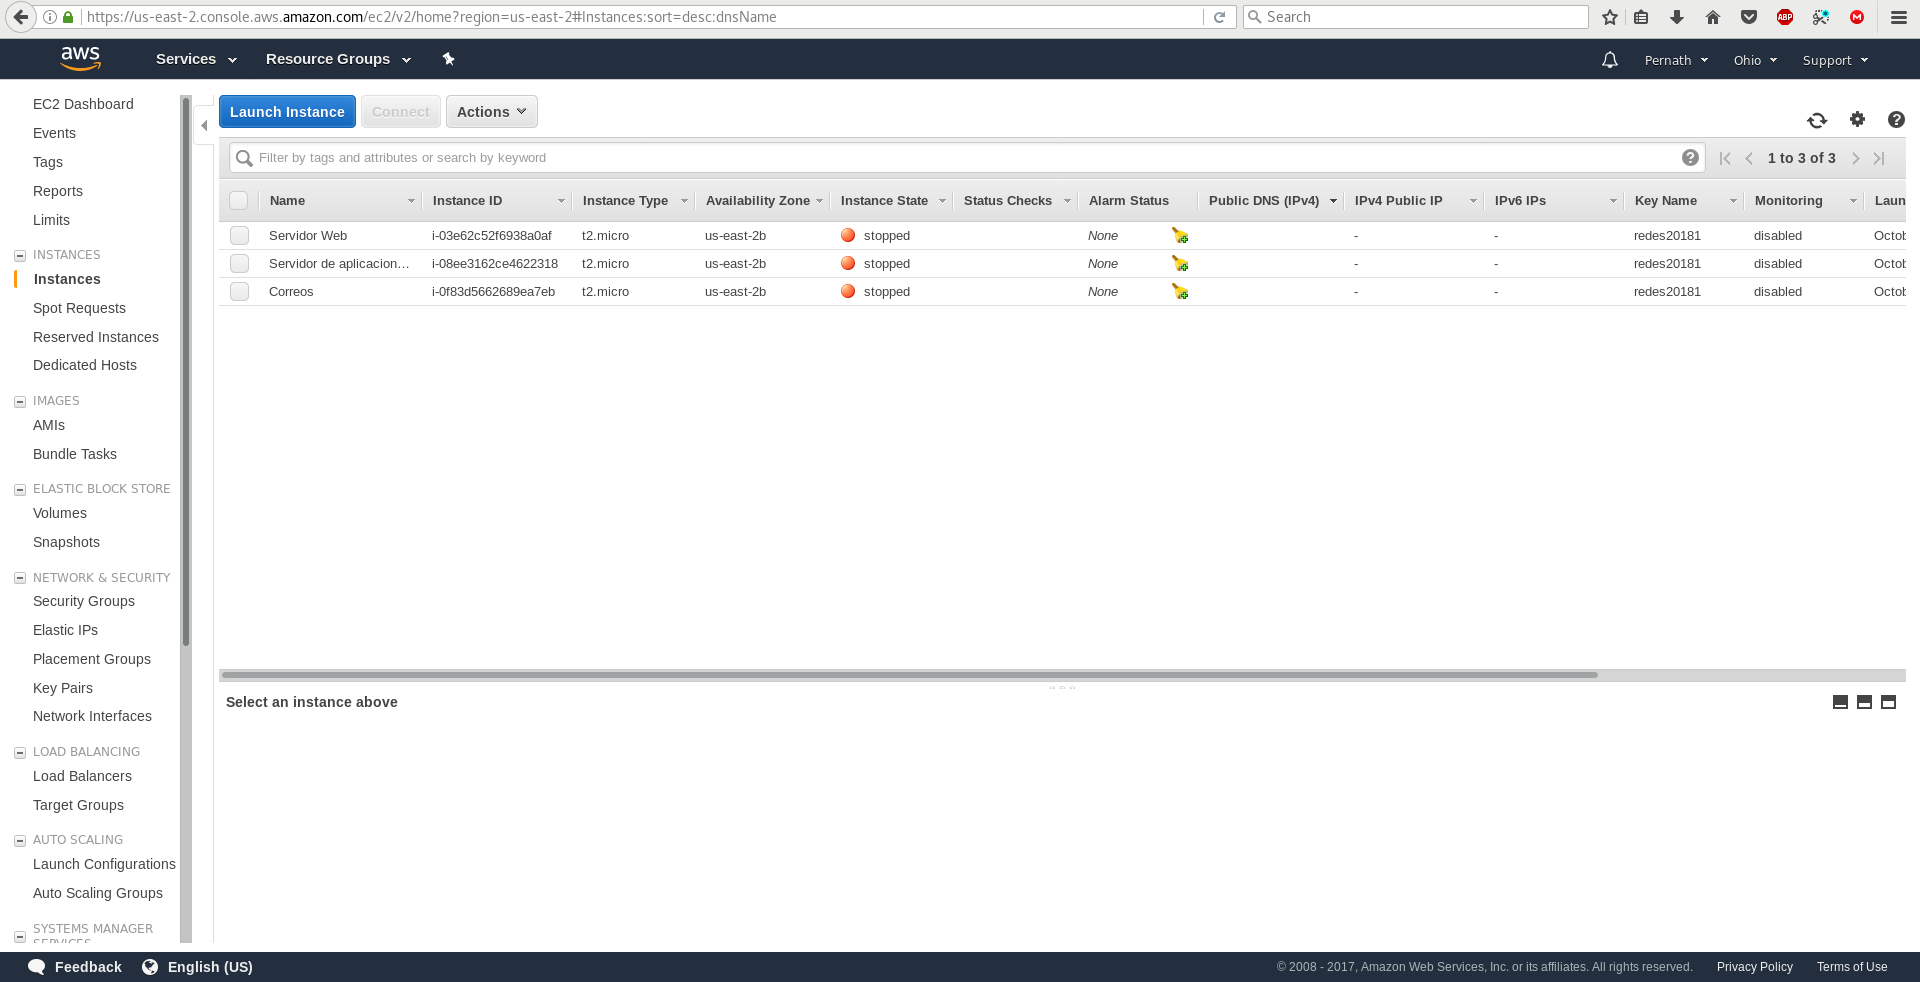
\includegraphics[width=\textwidth]{instances_dashboard}
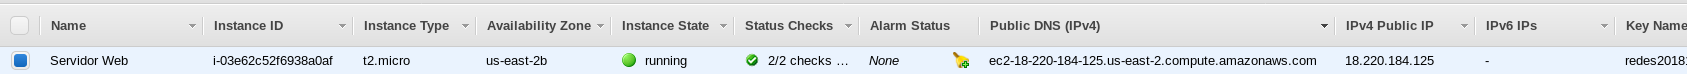
\includegraphics[width=\textwidth]{web_server}
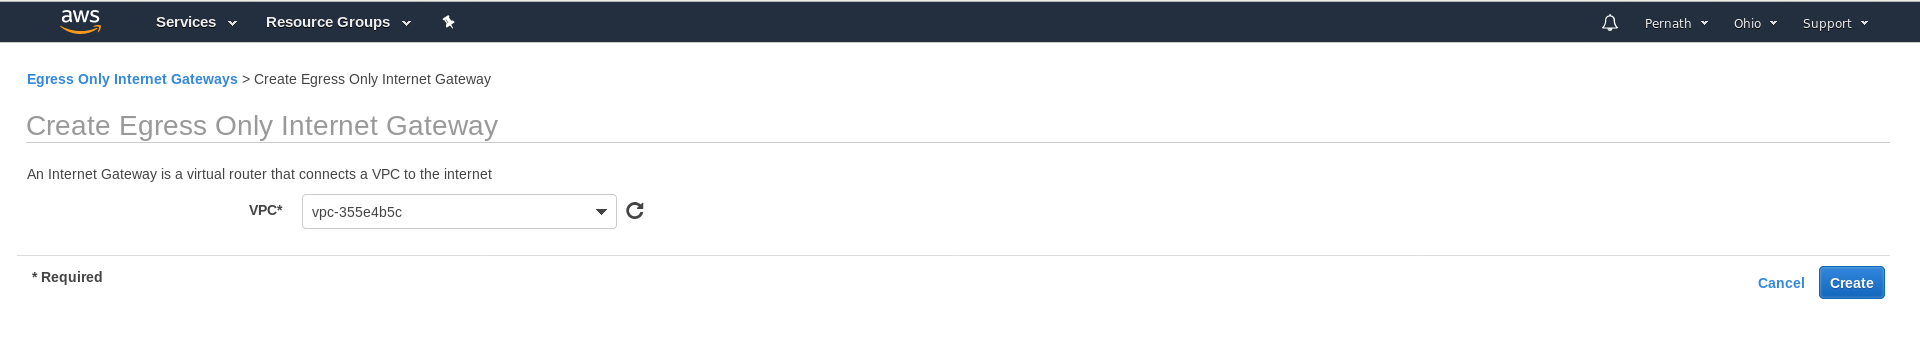
\includegraphics[width=\textwidth]{egress_only_gateway}
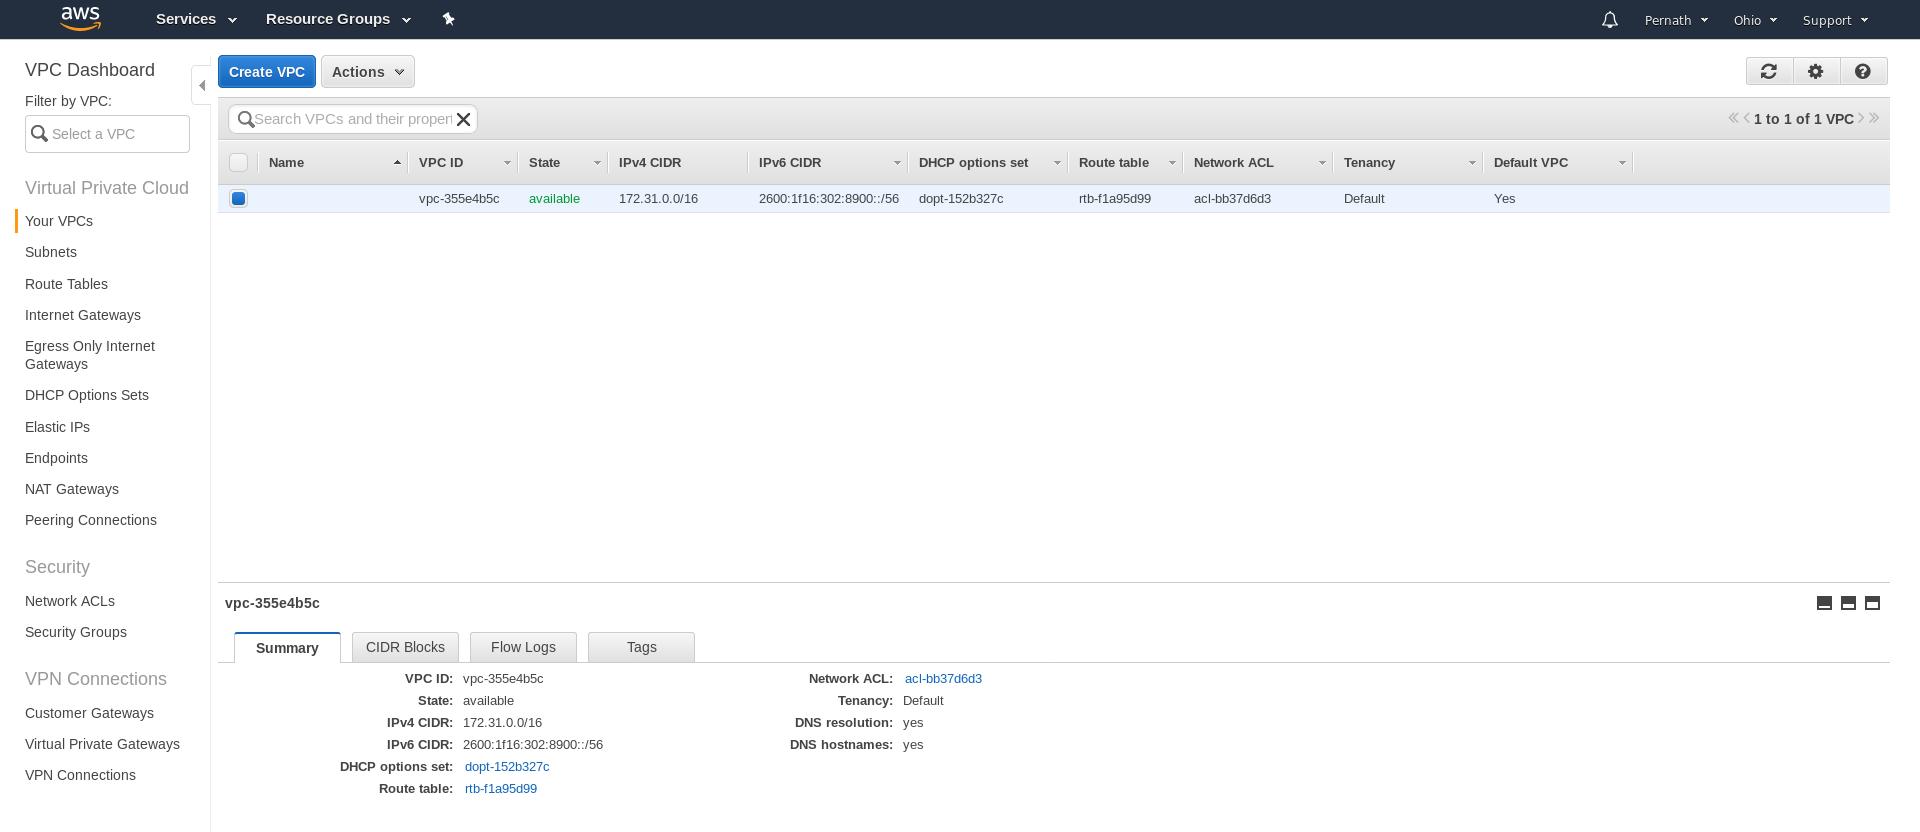
\includegraphics[width=\textwidth]{vpc}
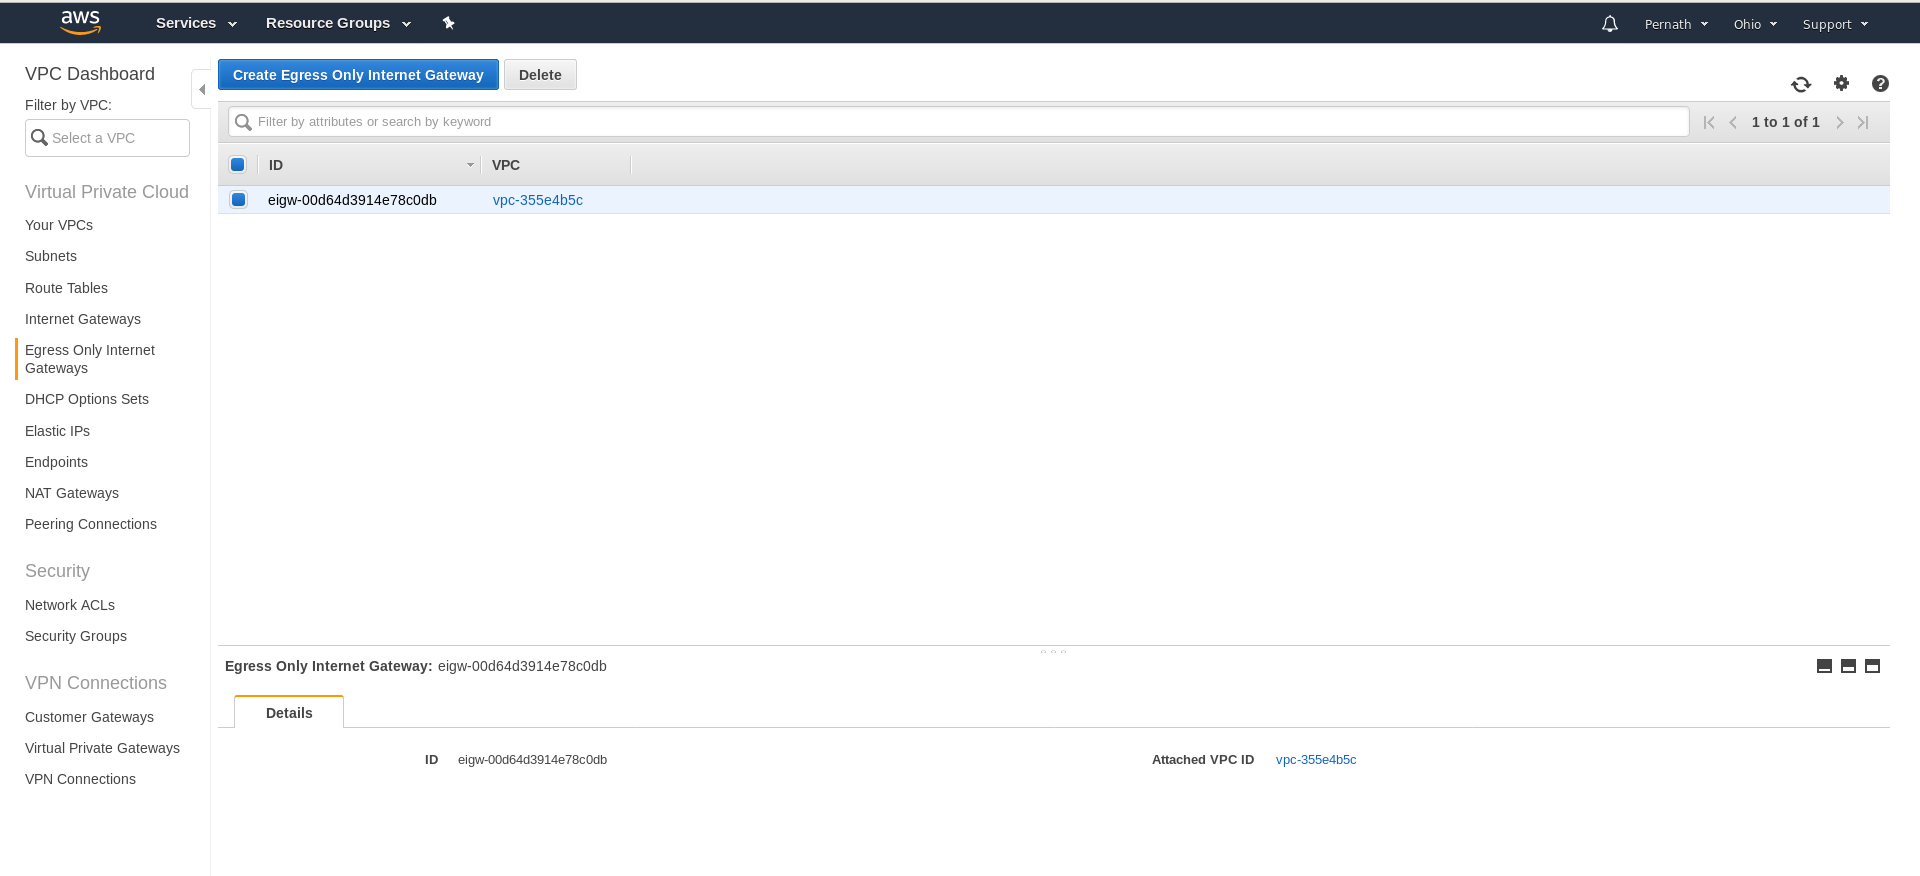
\includegraphics[width=\textwidth]{vpc_egress_only}
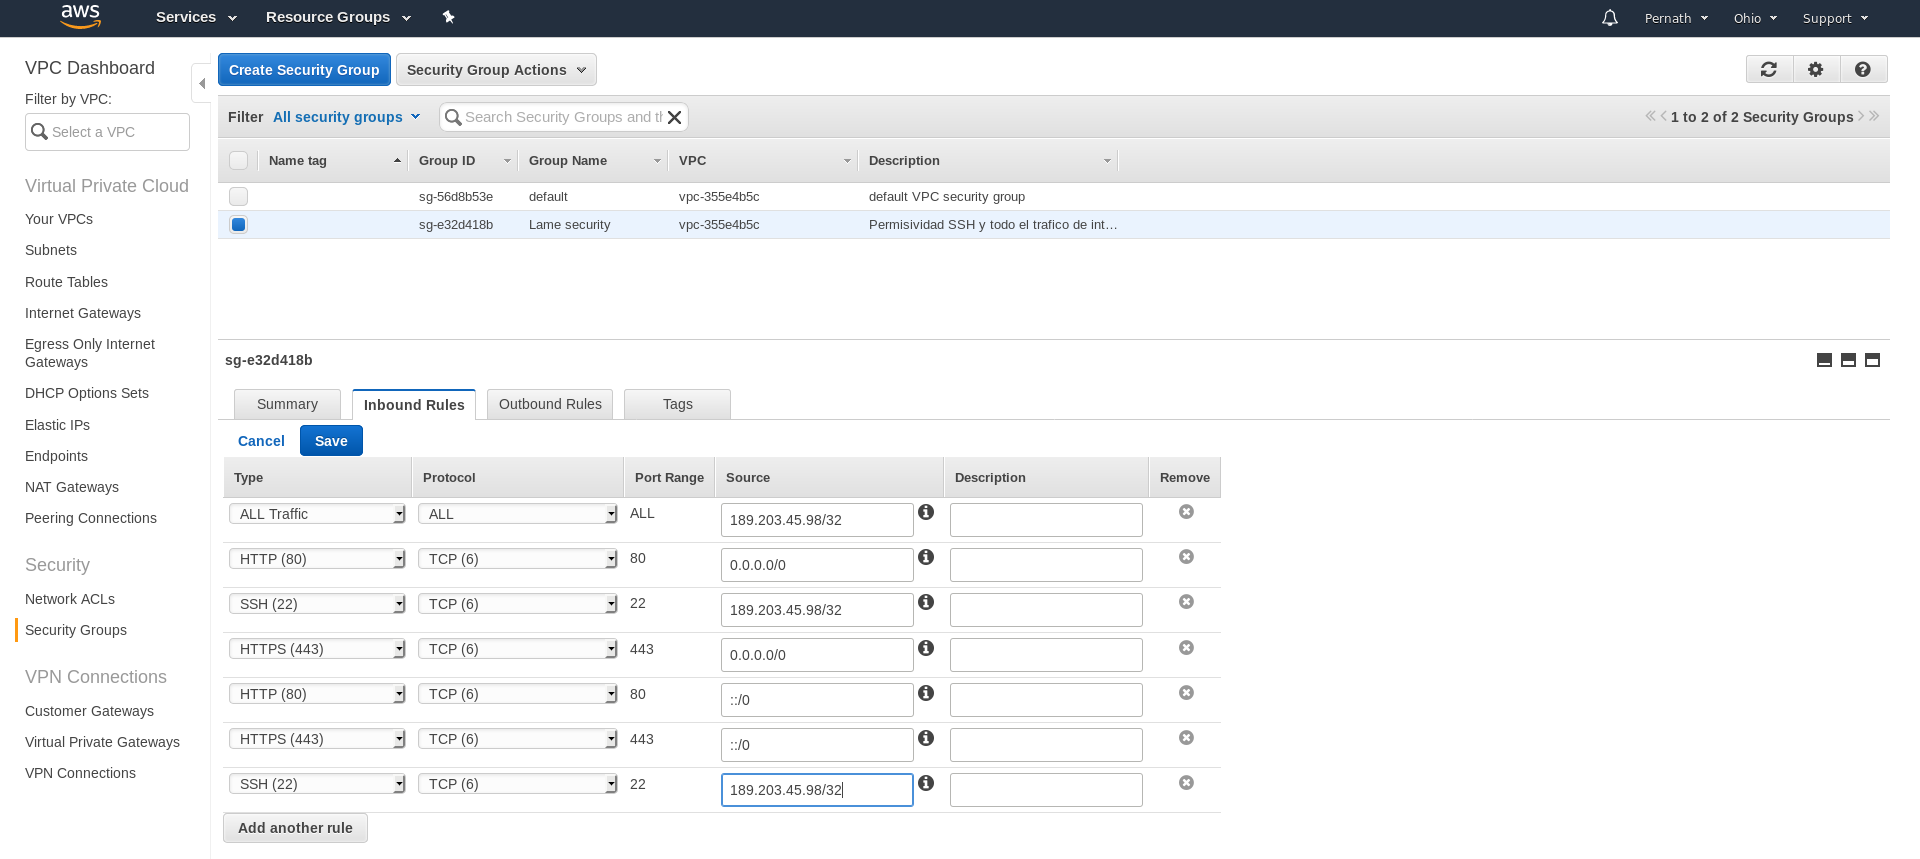
\includegraphics[width=\textwidth]{edit_security_group}
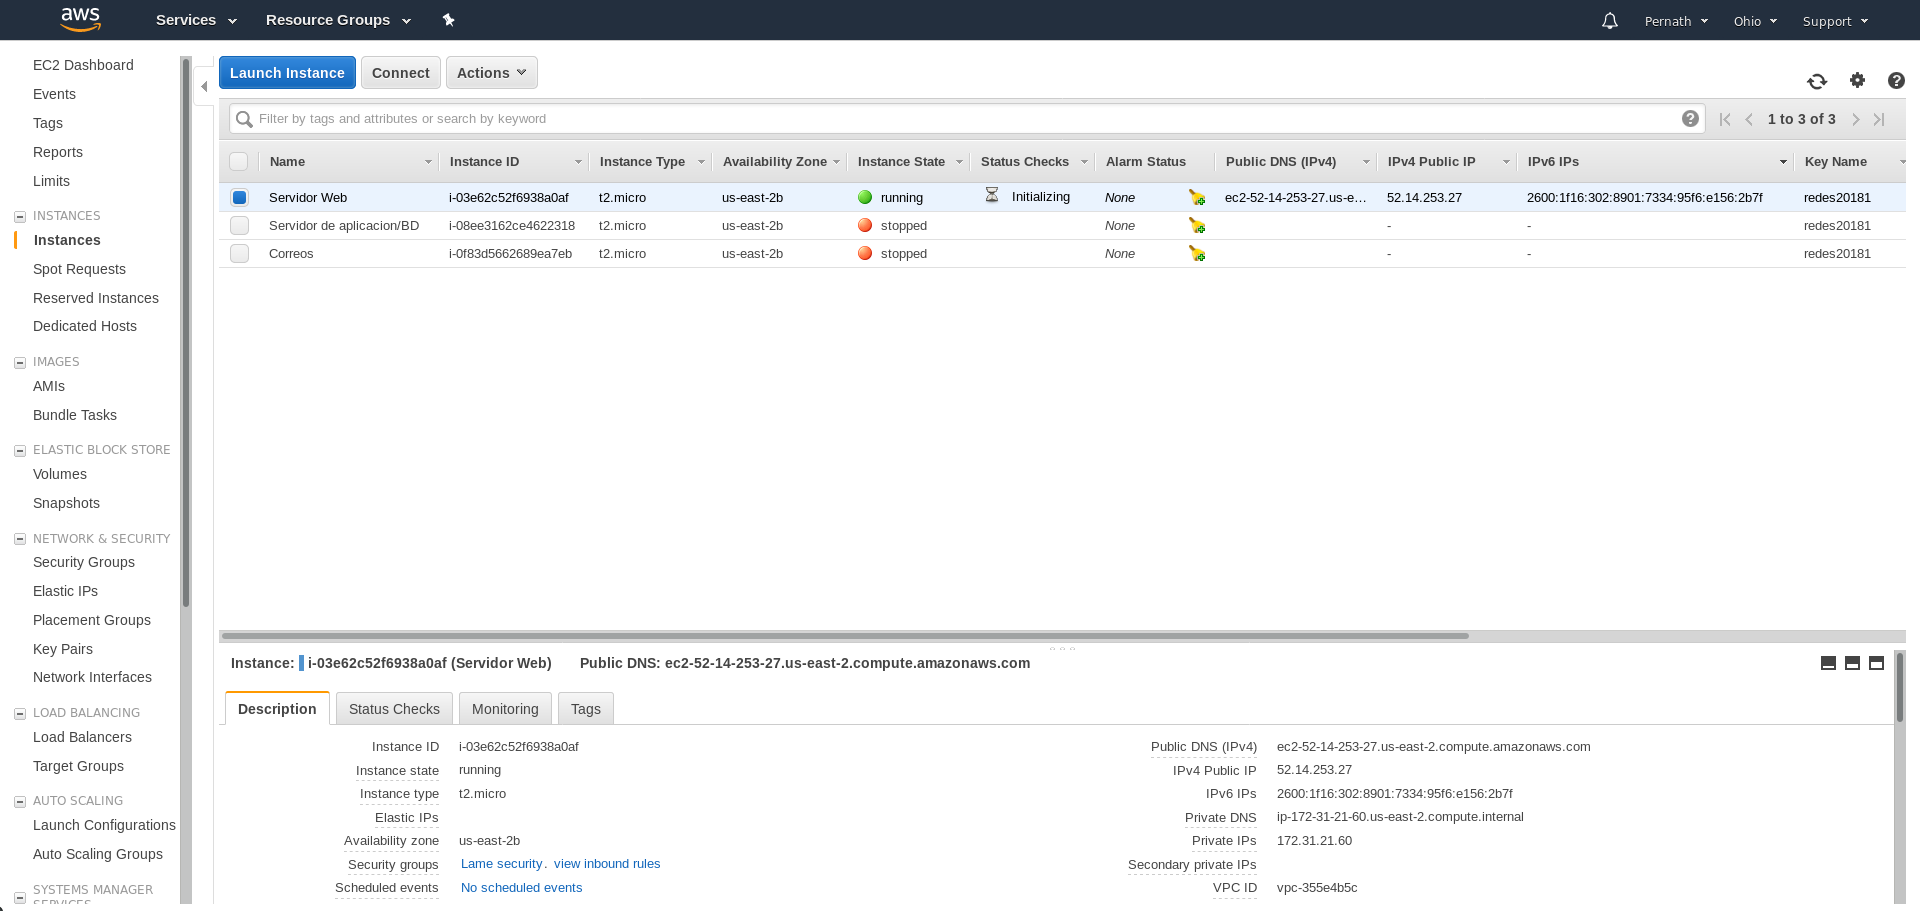
\includegraphics[width=\textwidth]{ipv6_assignment}
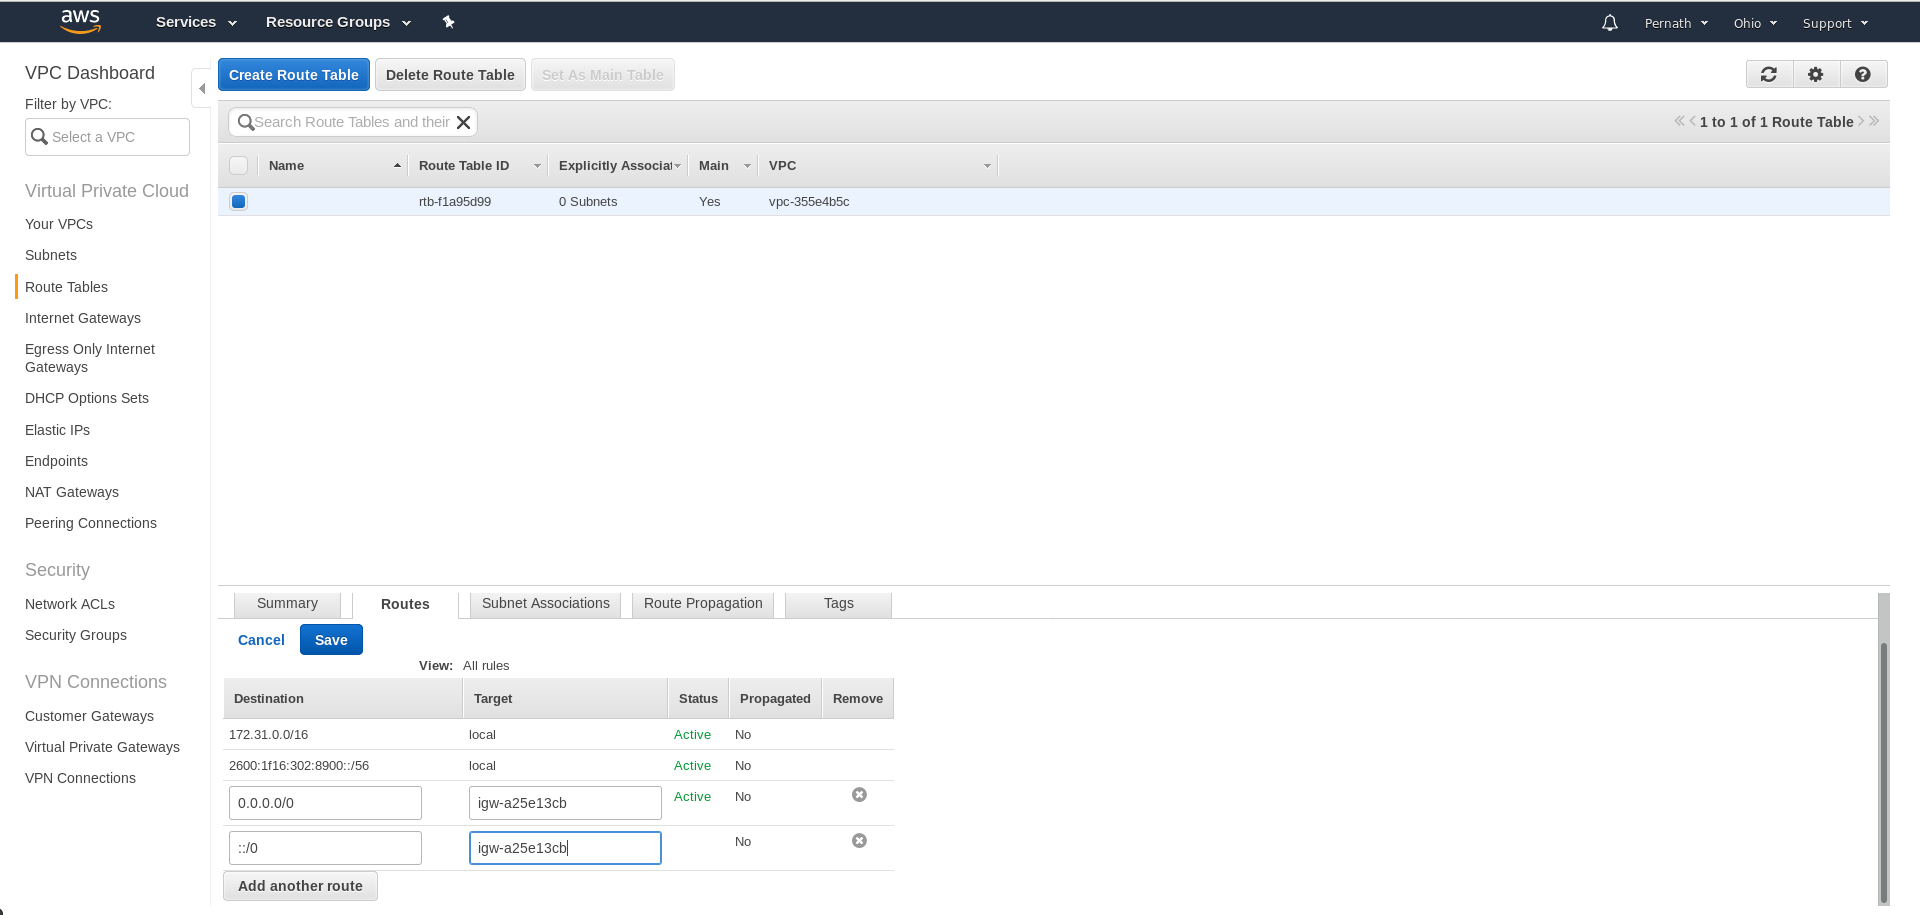
\includegraphics[width=\textwidth]{public_subnet}
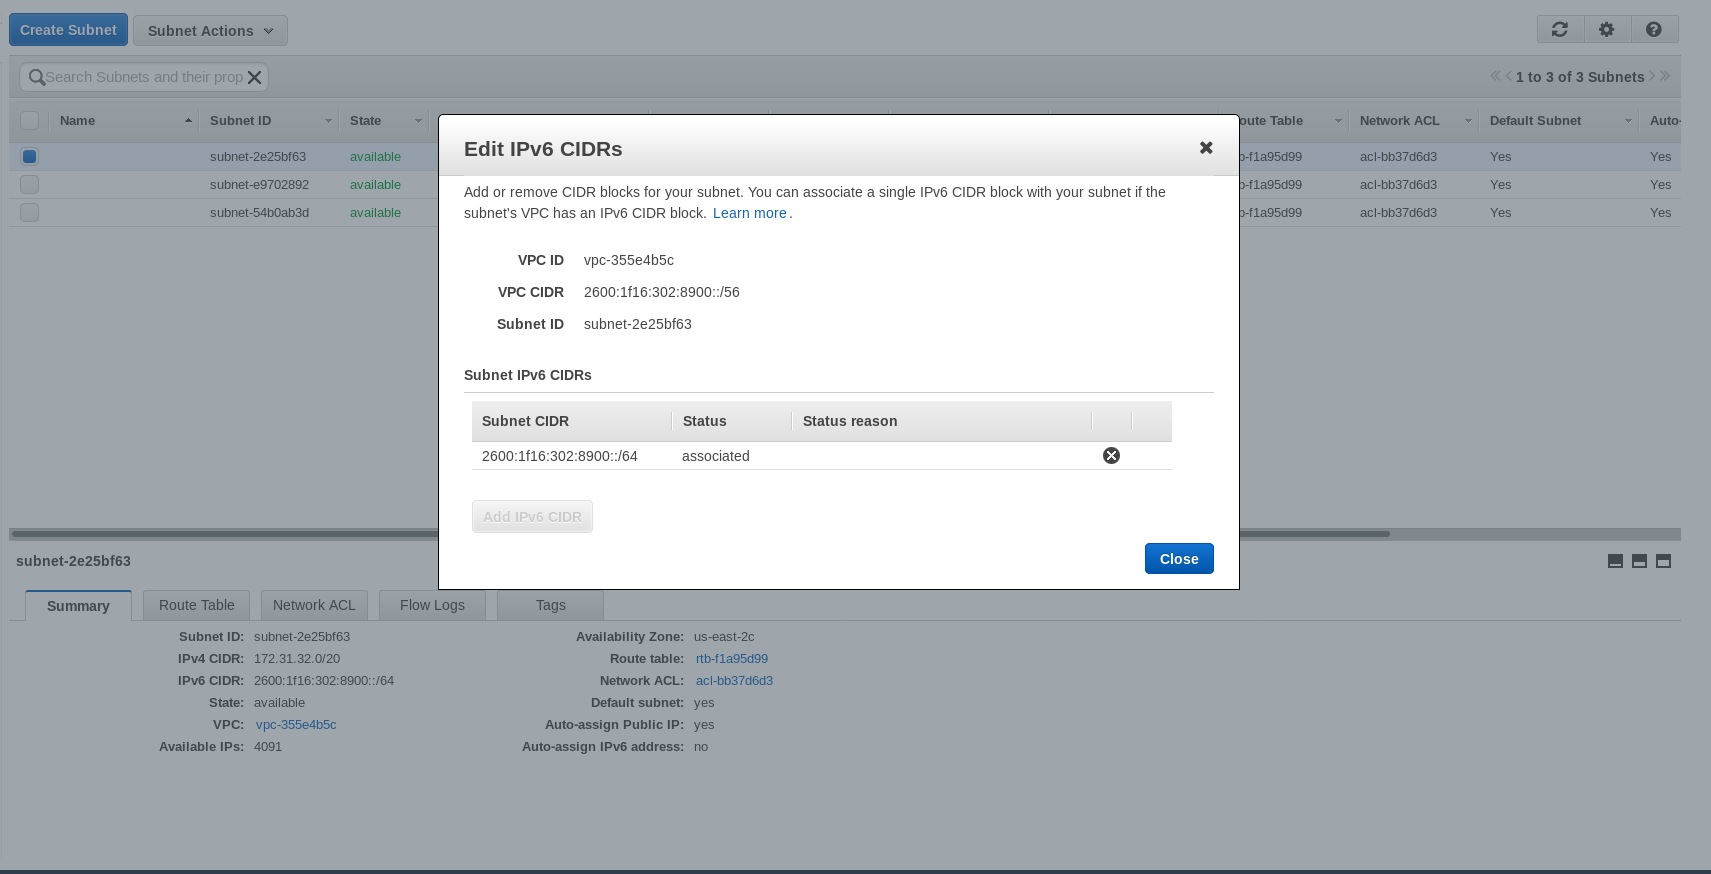
\includegraphics[width=\textwidth]{ipv6_cidr}
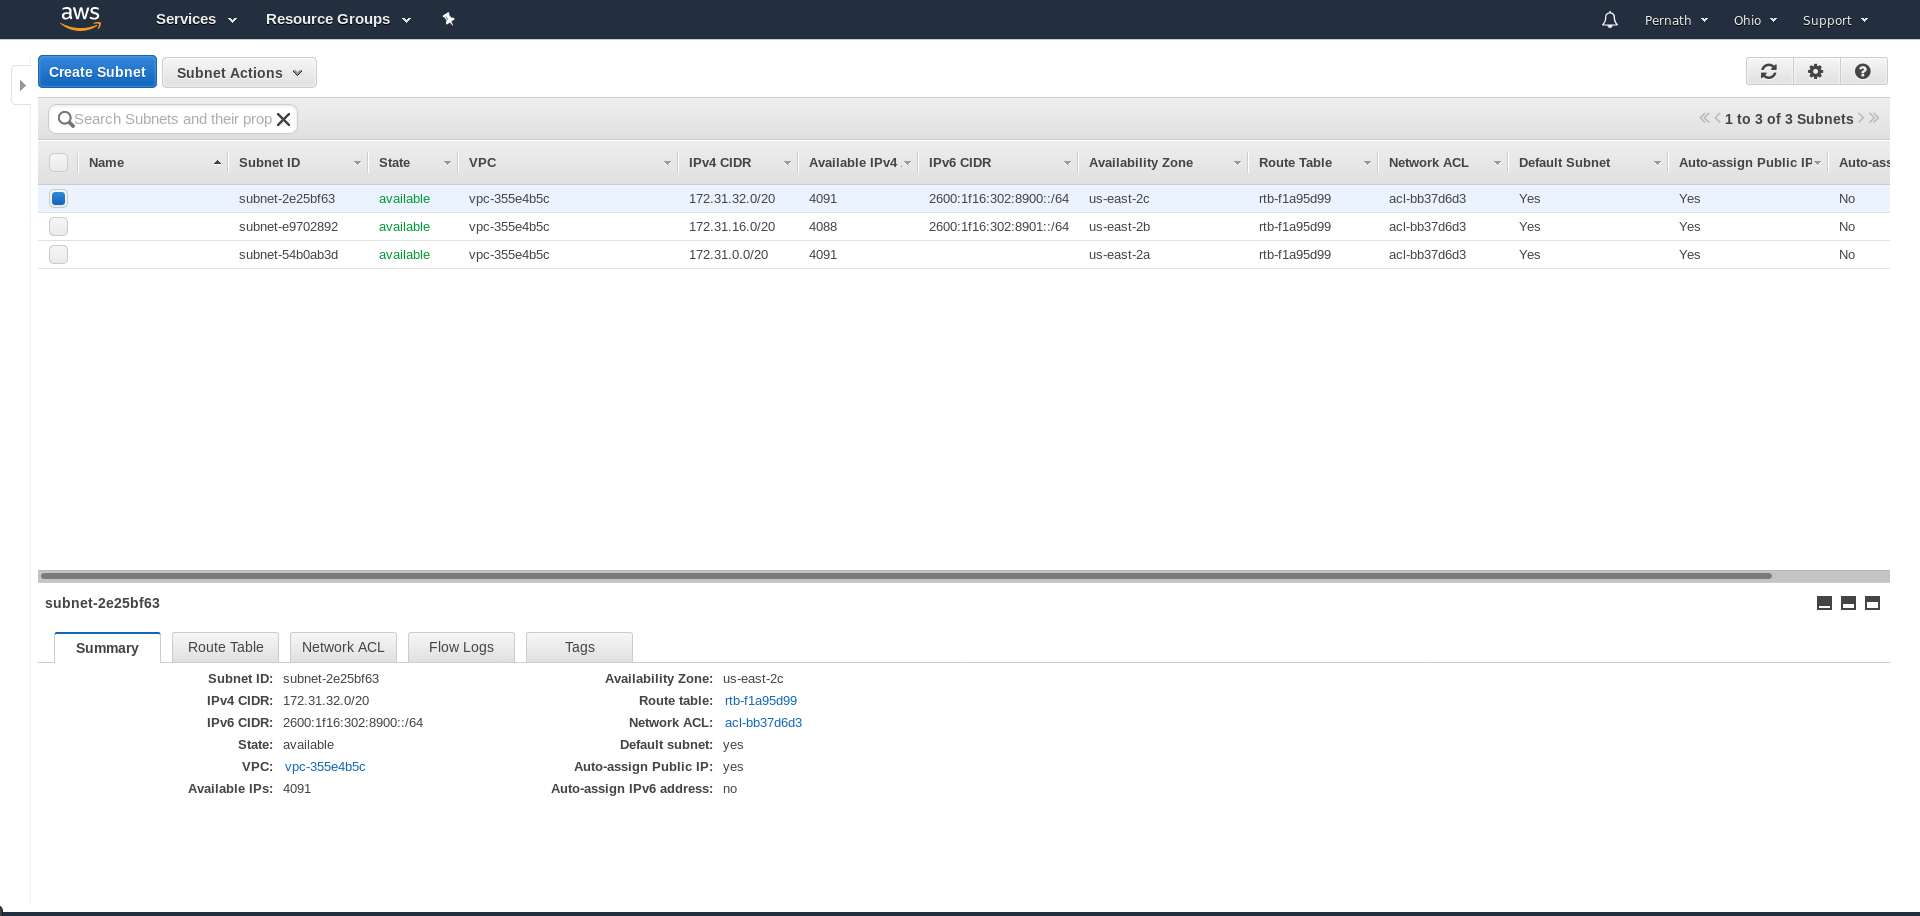
\includegraphics[width=\textwidth]{subnets}
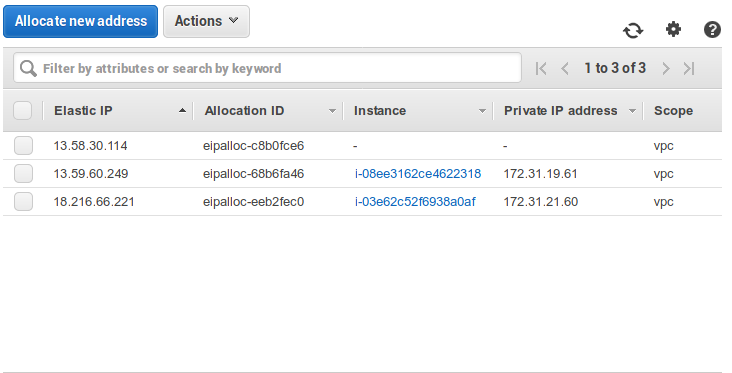
\includegraphics[width=\textwidth]{elastic_ip}
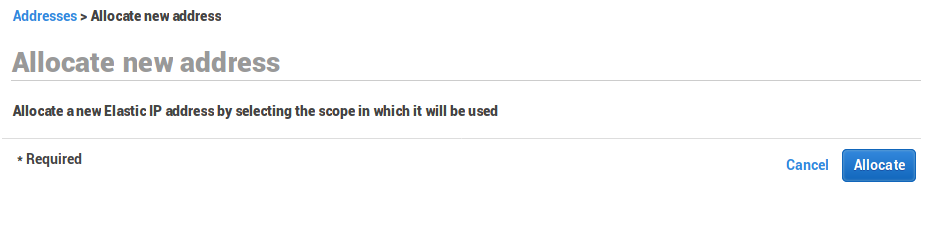
\includegraphics[width=\textwidth]{elastic_ip_allocate}
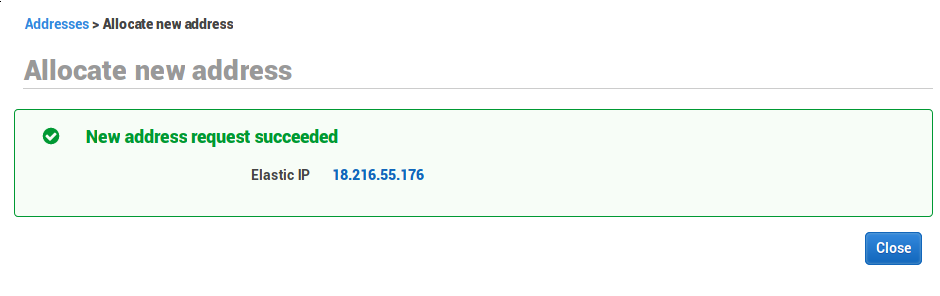
\includegraphics[width=\textwidth]{elastic_ip_success}
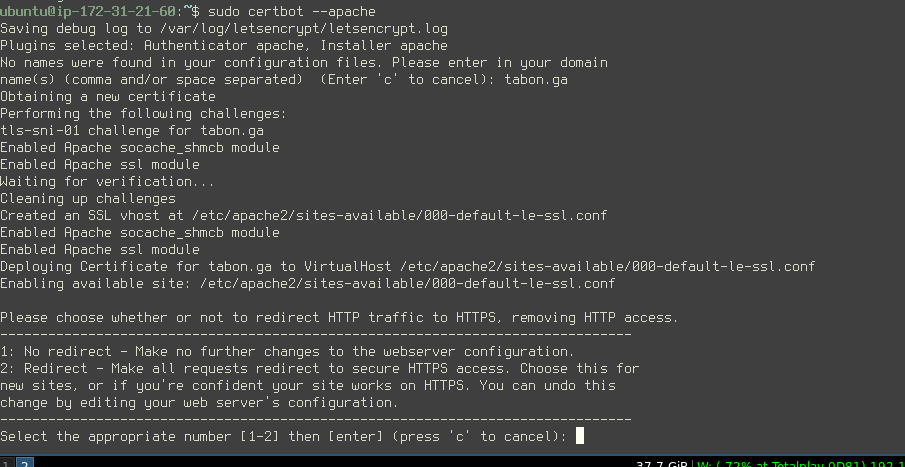
\includegraphics[width=\textwidth]{cert1}
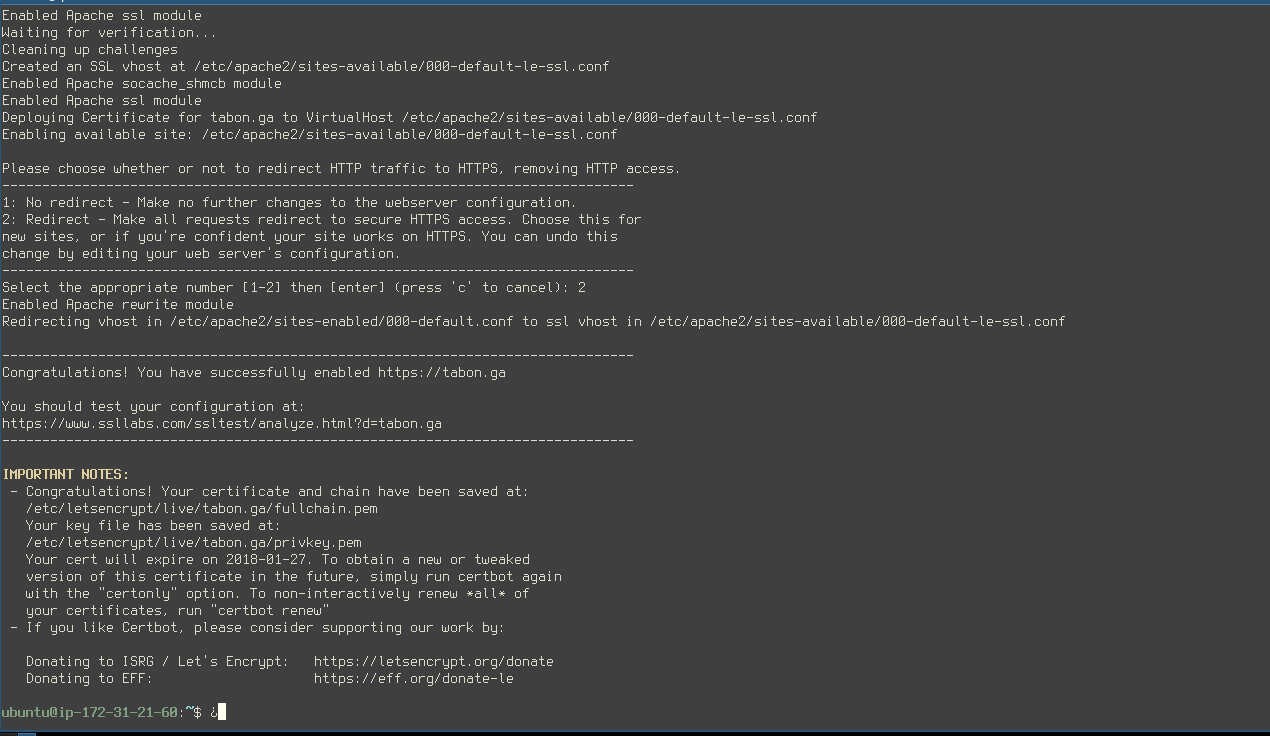
\includegraphics[width=\textwidth]{cert2}
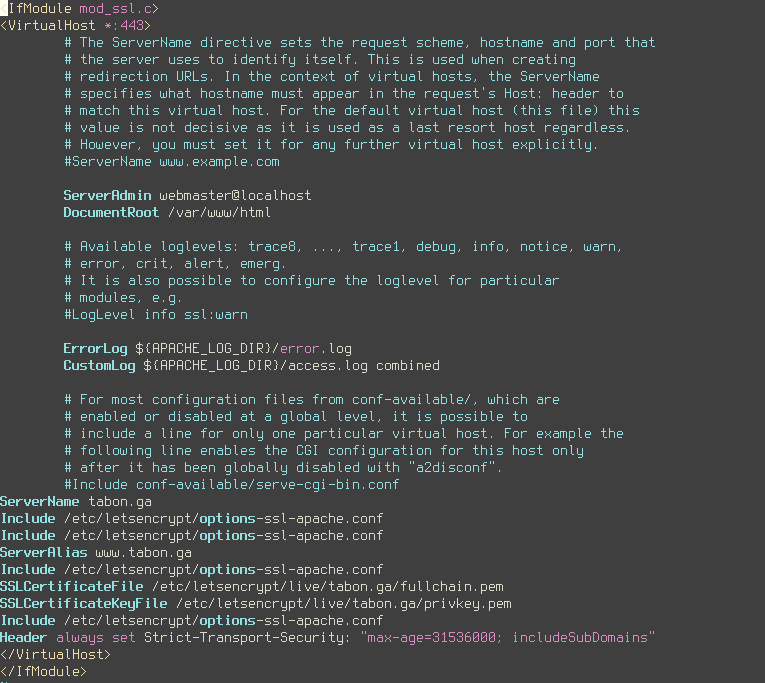
\includegraphics[width=\textwidth]{apache-ssl}
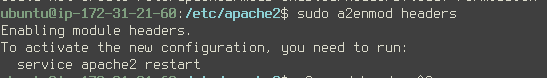
\includegraphics[width=\textwidth]{mods}
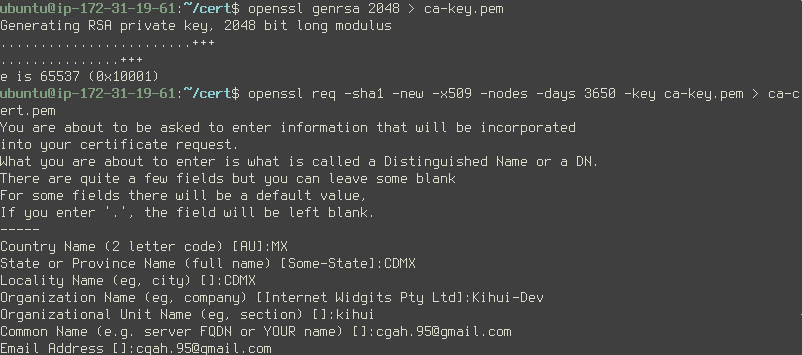
\includegraphics[width=\textwidth]{mysql_cert}
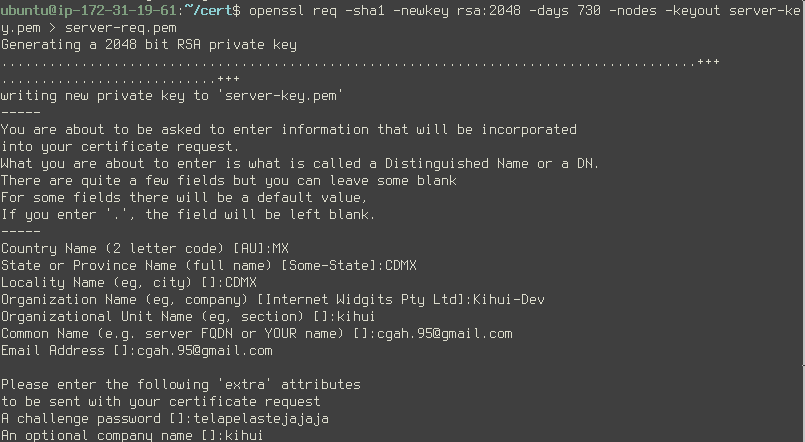
\includegraphics[width=\textwidth]{mysql_server-key}
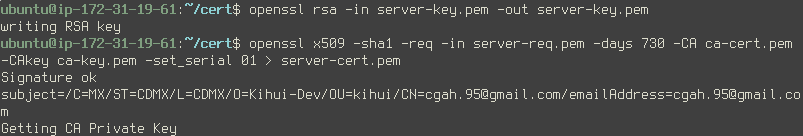
\includegraphics[width=\textwidth]{mysql_server-cert}
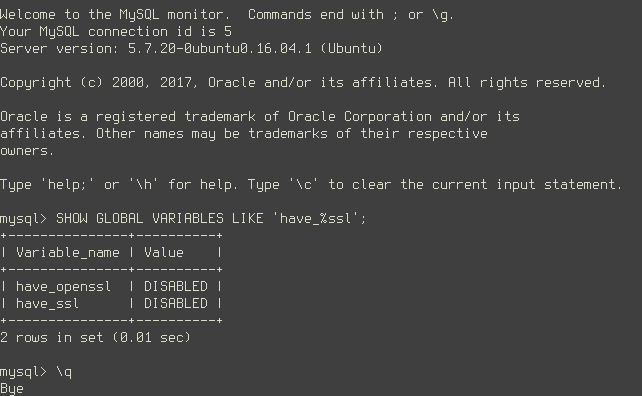
\includegraphics[width=\textwidth]{mysql_ssl-disabled}
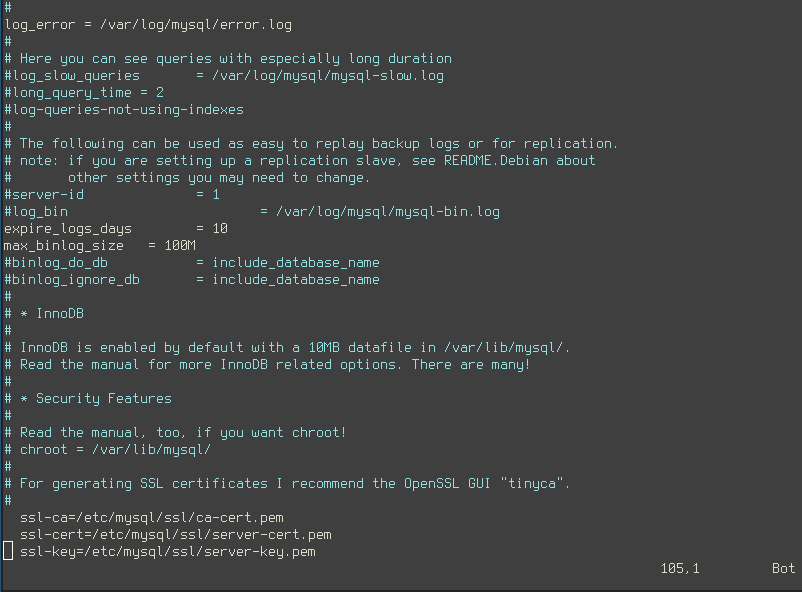
\includegraphics[width=\textwidth]{mysql_conf-ssl}
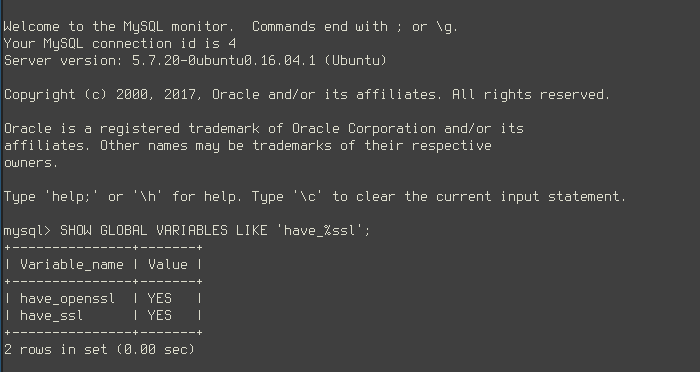
\includegraphics[width=\textwidth]{mysql_ssl-enabled}

\subsection*{Diagrama de la base de datos}
Dada la simpleza de la aplicación, la base de datos solo cuenta con una tabla para los usuarios con sus respectivos atributos.\\
\begin{figure}[h!]
  \centering
  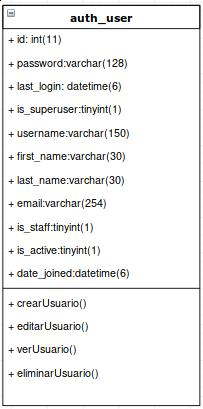
\includegraphics[scale=0.5]{db}
  \caption{Tabla de usuario}
\end{figure}

\subsection*{Objetivo de la aplicación}
La aplicación fue desarrollada con el fin de ilustrar las funciones básicas de una aplicación web con base de datos, es decir, \textit{crear, editar, ver y liminar} y que pueden asociarse a distintos métodos \textsf{HTTP} de la capa de aplicación como \textsf{PUT, POST, GET, PATCH o DELETE}. \\
A partir de esta pequeña aplicación \textit{CRUD} puede escalarse a proyectos más grandes y de mayor complejidad gracias a la escalabilidad de \textbf{Django}, el framework usado.

\subsection*{Uso de la aplicación}
Al ingresar al sitio, el usuario se encontrará con dos enlaces: uno para registrarse en la plataforma y otro para iniciar sesión en ésta.
\begin{figure}[h!]
  \centering
  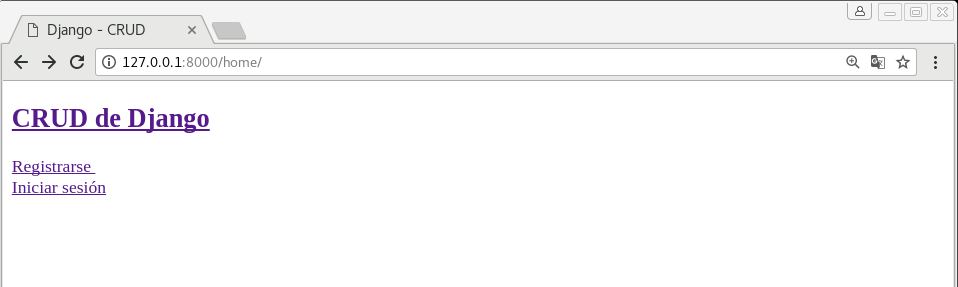
\includegraphics[width=\textwidth]{django_crud/home_notlogged}
  \caption{Página de inicio para usuarios sin sesión activa}
\end{figure}
\\
Si no está registrado e ingresa en el enlace para registrarse, será redireccionado a un formulario para que llene sus datos y se de de alta en la aplicación. 
\begin{figure}[h!]
  \centering
  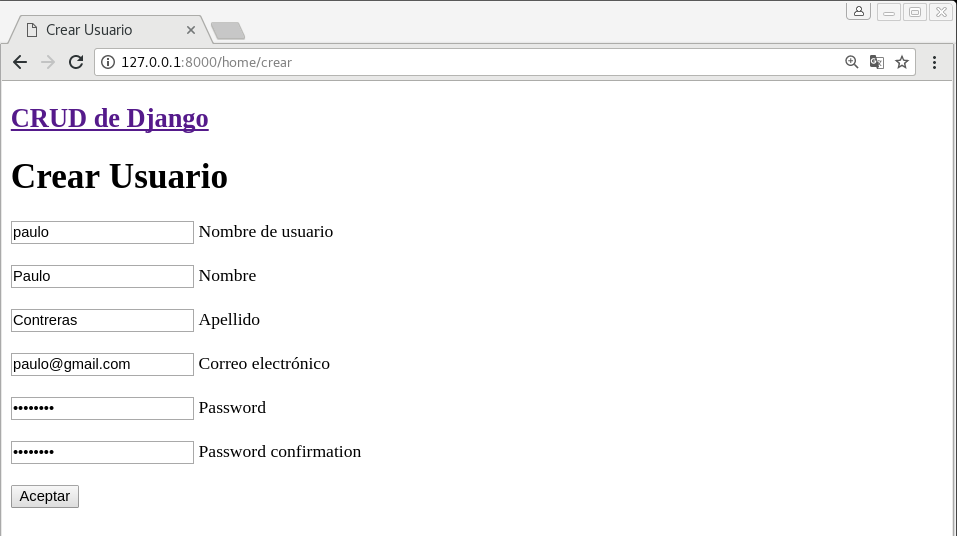
\includegraphics[width=\textwidth]{django_crud/registration}
  \caption{Formulario de registro para usuarios}
\end{figure}
\\
Si ya está registrado, podrá ingresar a la aplicación siguiendo el enlace de \textit{Iniciar sesión} en la página de inicio y en el formulario escribir el nombre de usuario y la contraseña con los que se registró.
\begin{figure}[h!]
  \centering
  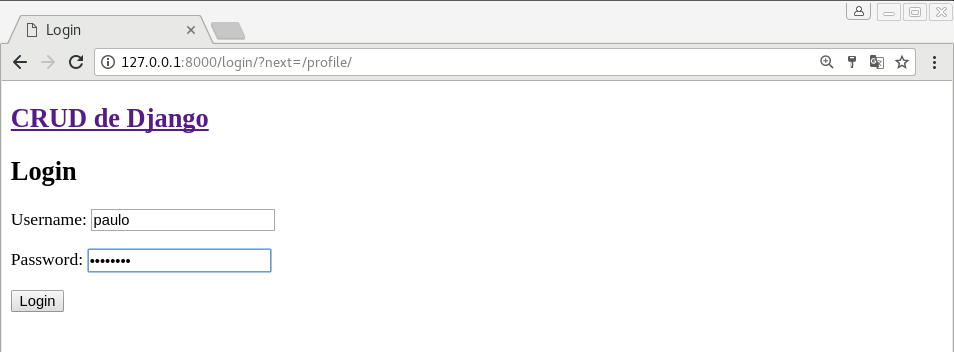
\includegraphics[width=\textwidth]{django_crud/login}
  \caption{Formulario de inicio de sesión}
\end{figure}
\\

Una vez dentro de la aplicación, el usuario verá una lista de los usuarios registrados y tendrá las opciones de ver información más detallada sobre algún usuario o sí mismo, actualizar sus datos o eliminar su cuenta si así lo desea.\\
\begin{figure}[ht!]
  \centering
  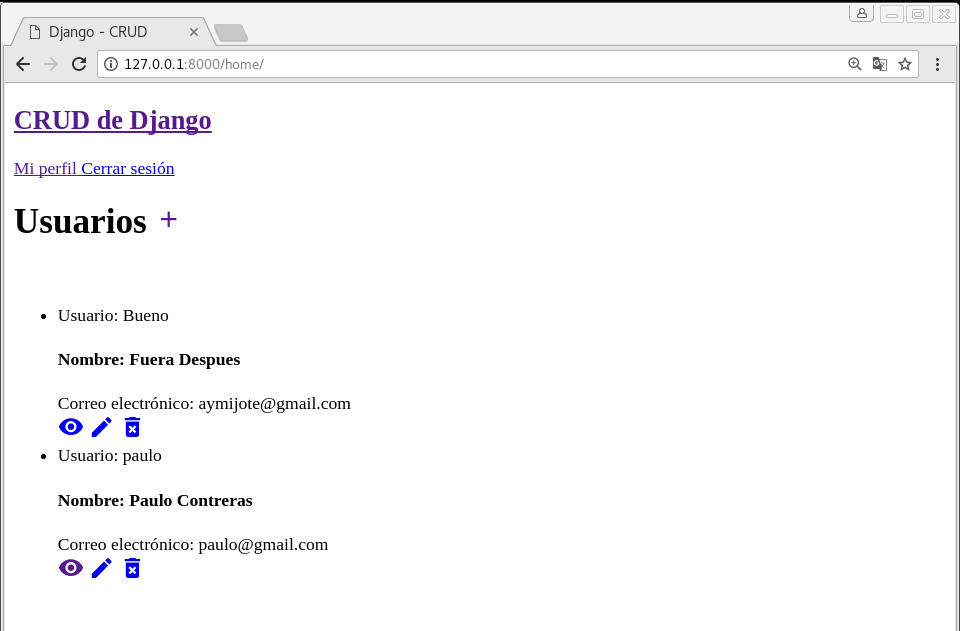
\includegraphics[width=\textwidth]{django_crud/home_logged}
  \caption{Página de inicio para usuarios con sesión activa}
\end{figure}
\\

Si elige ver información más detallada sobre un usuario, el enlace lo llevará al perfil del usuario. \\
\begin{figure}[ht!]
  \centering
  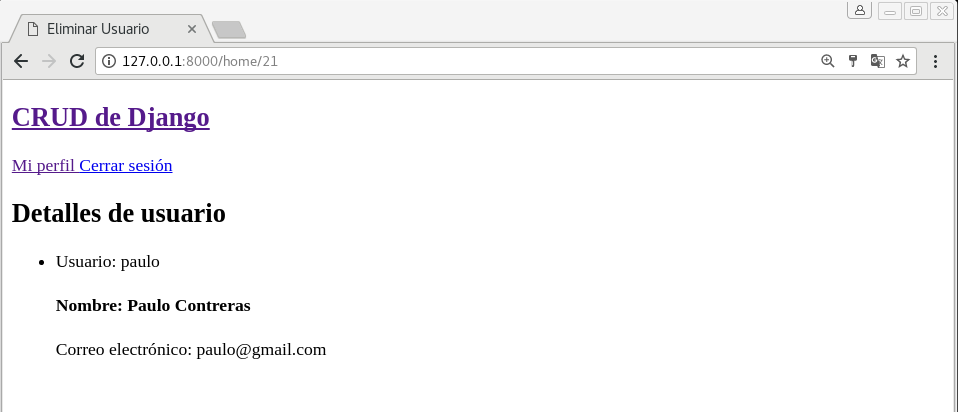
\includegraphics[width=\textwidth]{django_crud/profile}
  \caption{Perfil de usuario}
\end{figure}
\\

Para actualizar sus datos, será redirigido a un formulario similar al de registro.\\
\begin{figure}[ht!]
  \centering
  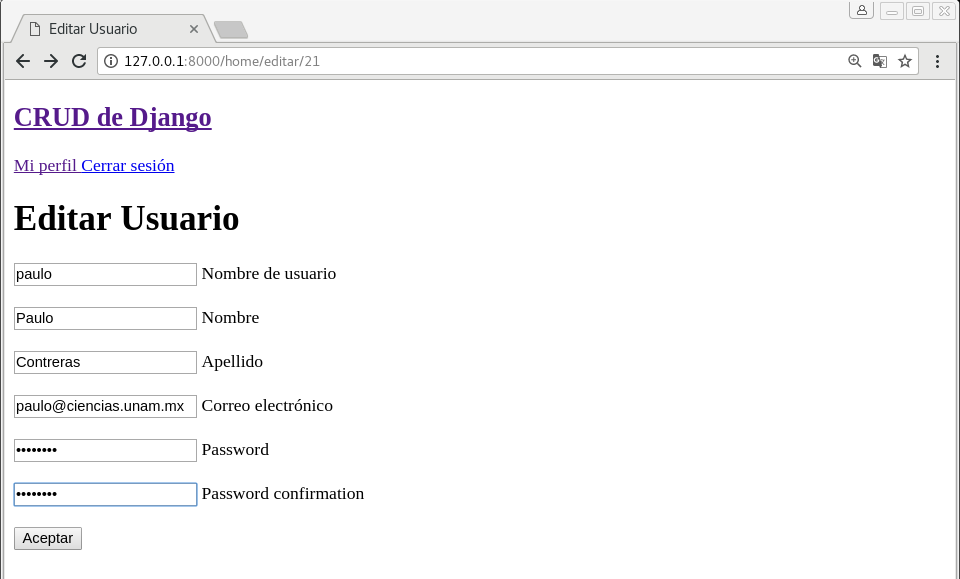
\includegraphics[width=\textwidth]{django_crud/update}
  \caption{Formulario de actualización de datos}
\end{figure}
\\

Si quiere eliminar su cuenta se le enviará un mensaje para que confirme su acción. \\
\begin{figure}[ht!]
  \centering
  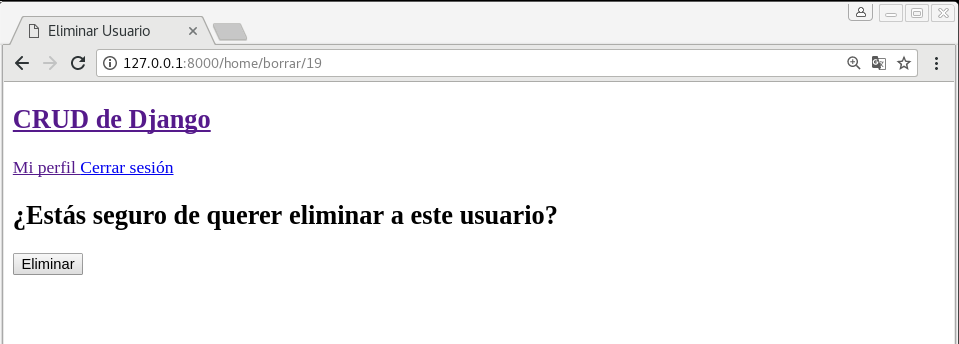
\includegraphics[width=\textwidth]{django_crud/delete}
  \caption{Mensaje de confirmación de eliminación de un usuario}
\end{figure}

\subsection*{Comentarios sobre el desarrollo del proyecto}
% We didn't deserve this
Intentamos hacer una aplicación lo más sencilla posible, minimizando la carga de trabajo que podría tener el servidor de aplicación, para enforcarnos en los aspectos más importantes que requería el proyecto: la comunicación entre los servidores y la seguridad en esta comunicación. %pero todo cambió cuando la nación del fuego atacó.

\end{document}
